% !TeX root = ../main.tex
\section{Reinitialize Bad Starts Study}
\label{sec:relu1-reinit}

\subsection*{Aim}
The baseline showed that plain Kaiming weights often leave at least one
XOR point \emph{inactive} for every neuron.  
Here we test a simple remedy: \textbf{re-initialise the network up to 100 times 
until all four inputs produce a positive pre-activation in \emph{each} ReLU}, 
using Kaiming-normal initialization with weights \(\sim \mathcal{N}(0, \sigma)\) and bias \(0\), as in Section~\ref{sec:relu1-kaiming}.
The reinitialization ensure that the network begins training without any dead data.
A second variant tightens the criterion by requiring a \emph{margin}
of $0.3$ in activation space.

\begin{description}[leftmargin=2em,style=sameline]
  \item[\texttt{relu1\_reinit}]   stop once \(\max_k f_k(x_i) > 0\) for every \(x_i\);
  \item[\texttt{relu1\_reinit\_margin}] stop once each \(x_i\) satisfies
        \(\max_k f_k(x_i) > 0.3\).
\end{description}
Both use the same optimiser and early-stop rules as previous sections.

% ------------------------------------------------------------------
\subsection*{Classification Accuracy}

\begin{table}[ht]
\centering
\caption{Final accuracy across runs.}
\label{tab:relu1-reinit-accuracy}
\begin{tabular}{lccccc}
\toprule
Variant & 0\,\% & 25\,\% & 50\,\% & 75\,\% & 100\,\% \\
\midrule
Baseline (ReLU)       & 0 & 0 & 0 & 26 & 24 \\
Reinit (no margin)    & 0 & 0 & 0 & 5  & 45 \\
Reinit + margin 0.3   & 0 & 0 & 0 & 4  & 496/500 \\
\bottomrule
\end{tabular}
\end{table}

\paragraph{Headline}
A single pass of dead-data re-init lifts success from
$48\,\%\!\to\!90\,\%$;
adding the $0.3$ margin pushes reliability to \(\approx99\,\%\).

% ------------------------------------------------------------------
\subsection*{Convergence Timing}

\begin{table}[ht]
\centering
\caption{Epochs to early-stop (successful runs only).}
\label{tab:relu1-reinit-epochs}
\begin{tabular}{lccccc}
\toprule
Variant & 0\,\% & 25\,\% & 50\,\% & 75\,\% & 100\,\% \\
\midrule
Reinit            & 26 & 119 & 168 & 233 & 336 \\
Reinit + margin   & 44 & 132 & 190 & 255 & 448 \\
\bottomrule
\end{tabular}
\end{table}

Median training time increases modestly under the margin rule because
the initial sampling occasionally needs several tries.

% ------------------------------------------------------------------
\subsection*{Hyperplane Geometry}

\begin{description}[leftmargin=2em]
  \item[Distance clusters] Both variants collapse to a \emph{single}
        distance pattern, as in the baseline, but the class-0 distances
        shift from \(0.29\pm0.20\) (no margin) to
        \(0.36\pm0.17\) with margin, reflecting the enforced offset.%
        
  \item[Weight clusters] Dead-data re-init reduces the number of weight
        clusters from nine (baseline) to seven; the margin variant
        compresses them to six with a dominant pair of mirror-centroids
        covering $>95\,\%$ of runs.%
  \item[Mirror symmetry] Mirror pairs rise from
        $37/50$ (74\,\%) to $442/500$ (88\,\%) and the count of
        \emph{perfect} mirrors almost doubles
        (11 → 94).%
\end{description}

\subsection*{Emergent Failure Modes}
A second failure pattern surfaces even after dead-data screening:
in rare cases hyperplanes fall into a local basin that is almost
\emph{perpendicular} to any solution-bearing orientation (example shown in Fig.\,\ref{fig:reinit-bad}).
These runs account for the residual $75\,\%$ accuracies in both tables. 
We notice that this hyperplane is also dead and does not intersect the data space.
It is not clear how the initial state relates to this basin.

\begin{figure}[ht]
  \centering
  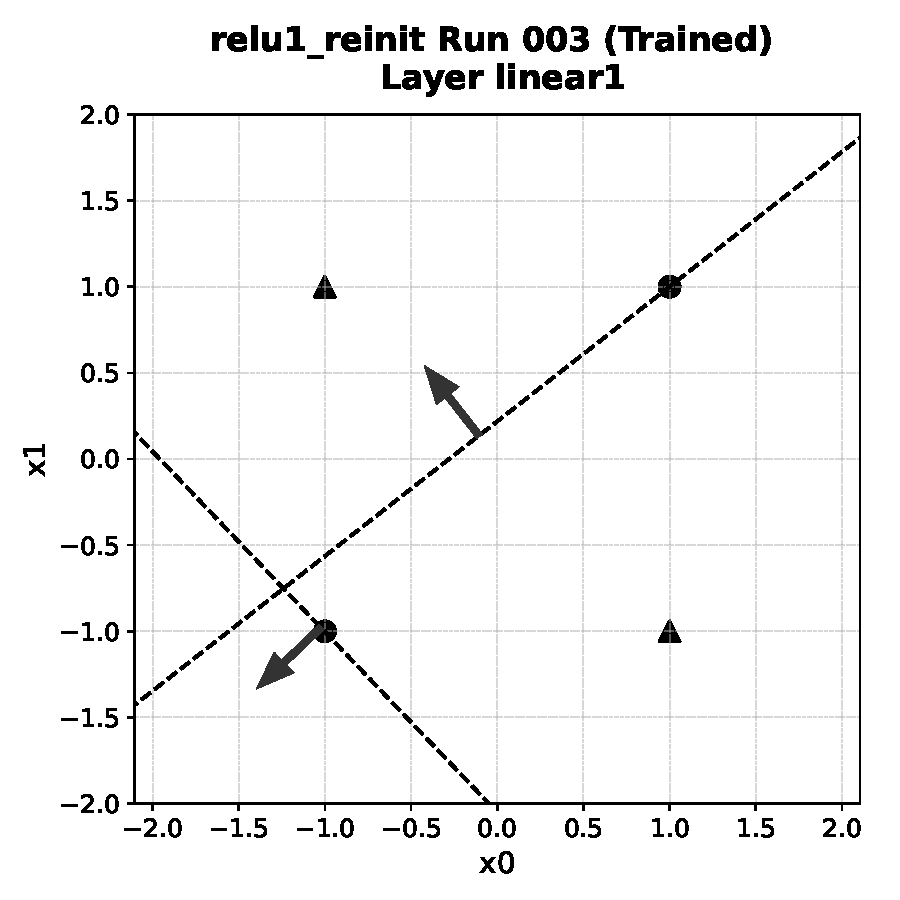
\includegraphics[width=0.38\textwidth]{relu1/figs/reinit_bad_example.pdf}
  \caption{Illustration of the "perpendicular" failure: the left dashed
           line rotates perpendicular to the optimal position.}
  \label{fig:reinit-bad}
\end{figure}

% ------------------------------------------------------------------
\paragraph{Discussion}
\begin{itemize}
  \item Screening out dead inputs at \emph{initialisation} is a
        lightweight, one-shot fix that triples the reliability of the
        two-ReLU model.
  \item Enforcing a small positive margin further reduces variance at the
        cost of extra sampling time, moving success toward certainty.
  \item Prototype-surface geometry tightens: mirror solutions dominate
        and distance clusters homogenise, reinforcing the theory's
        prediction that symmetry emerges once every input is alive.
  \item The remaining errors stem from a distinct "dying-ReLU" 
        trap, which motivates the runtime monitors discussed next.
\end{itemize}

\hrulefill
